\documentclass{article}

\usepackage{array}
\usepackage[utf8]{inputenc}
\usepackage[margin=1in]{geometry}
\usepackage[english]{babel}
\renewcommand{\baselinestretch}{1.2} % line spacing
\usepackage{graphicx} % for figures
\usepackage{caption} % for sub-figure
\usepackage{subcaption}% for sub-figure

\title{D4 Team Report}
\author{mi3g15 }
\date{March 2017}

\begin{document}

\maketitle

\section{Final Product Section}
Table for comparison of achievements with the tasked specifications:
\begin{center}
  \begin{table}
    \begin{tabular}{|m{5cm}|m{8cm}|}
    \hline
     Specifications & Achievements \\
     \hline
     Arming system for the motors to ensure safety compliance &  We made 4 propeller guards from reusable coat hangers by reshaping it to the right size and dimension and were proven to be reliable and cost effective.\\
    \hline
    Motor speed controlled by 1-2ms PWM ESCs - $I_{max}$:20 A & Achieved higher resolution of motor speed control within 125-250us using high resolution timers from the Leonardo.\\
    \hline
    RF modules operated using SPI Interface & %Achieved by using the rfm12 library from online source which establishes SPI interface with the Il Matto boards. 
    Achieved this since we were able to receive data that was transmitted from base station Il Matto to drone Il Matto. This proves that the SPI works reliably for sending and retrieving data between the Il Matto and the RF modules.\\
    \hline
    On-board file logging to SD card & Unable to achieve due to lack of time and coding issues with writing data to the SD card. \\
    \hline
    I2C interface at 100 samples per sec with Gyroscope and accelerometer(MPU6050) with built in DMP & Achieved reading data from this sensor at the specified rate.  \\
    \hline
    Servo used for cargo acquisition- controlled by PWM & Achieved control of servo using PWM. \\
    \hline
    Laser-cut acrylic chassis and assembled using acrylic glue & Achieved successful construction for initial and final chassis designs. \\
    \hline 
    I-style design for easier weight distribution and more carrying capacity & Achieved implementing this chassis design but in the final product, we added 'I' supports to the centre as well as to the arms to make the chassis more robust to object/ground collision. \\
    \hline
    Reprogram the PID controller on the fly by changing K values wirelessly for faster tuning & Program has been developed on the base station to send k values but has be modified for sending these values while the drone is on ground only. Also this method of re-tuning has not be used due to risk of a fault in wireless up-link and limited time for tuning of the PID controller.\\
    \hline
    Interfaced with the pilot using two X-Y joystick potentiometers, a bank of function switches, and a micro-controller & Achieved a remote controller module consisting of these components which has been designed, programmed and tested.\\
    \hline 
    Sharp GP2Y0A41SK0F IR sensor providing altitude sensing for telemetry with accuracy from 15 to 100cm & Sensor has shown to work reliably for the specified range and also implemented receiving IR sensor data for telemetry.\\
    \hline
    \end{tabular}
    \caption{Table comparing the Specification to the Achieved results}
  \end{table}
\end{center}
\begin{figure}[t]
    \begin{subfigure}{0.5\textwidth}
    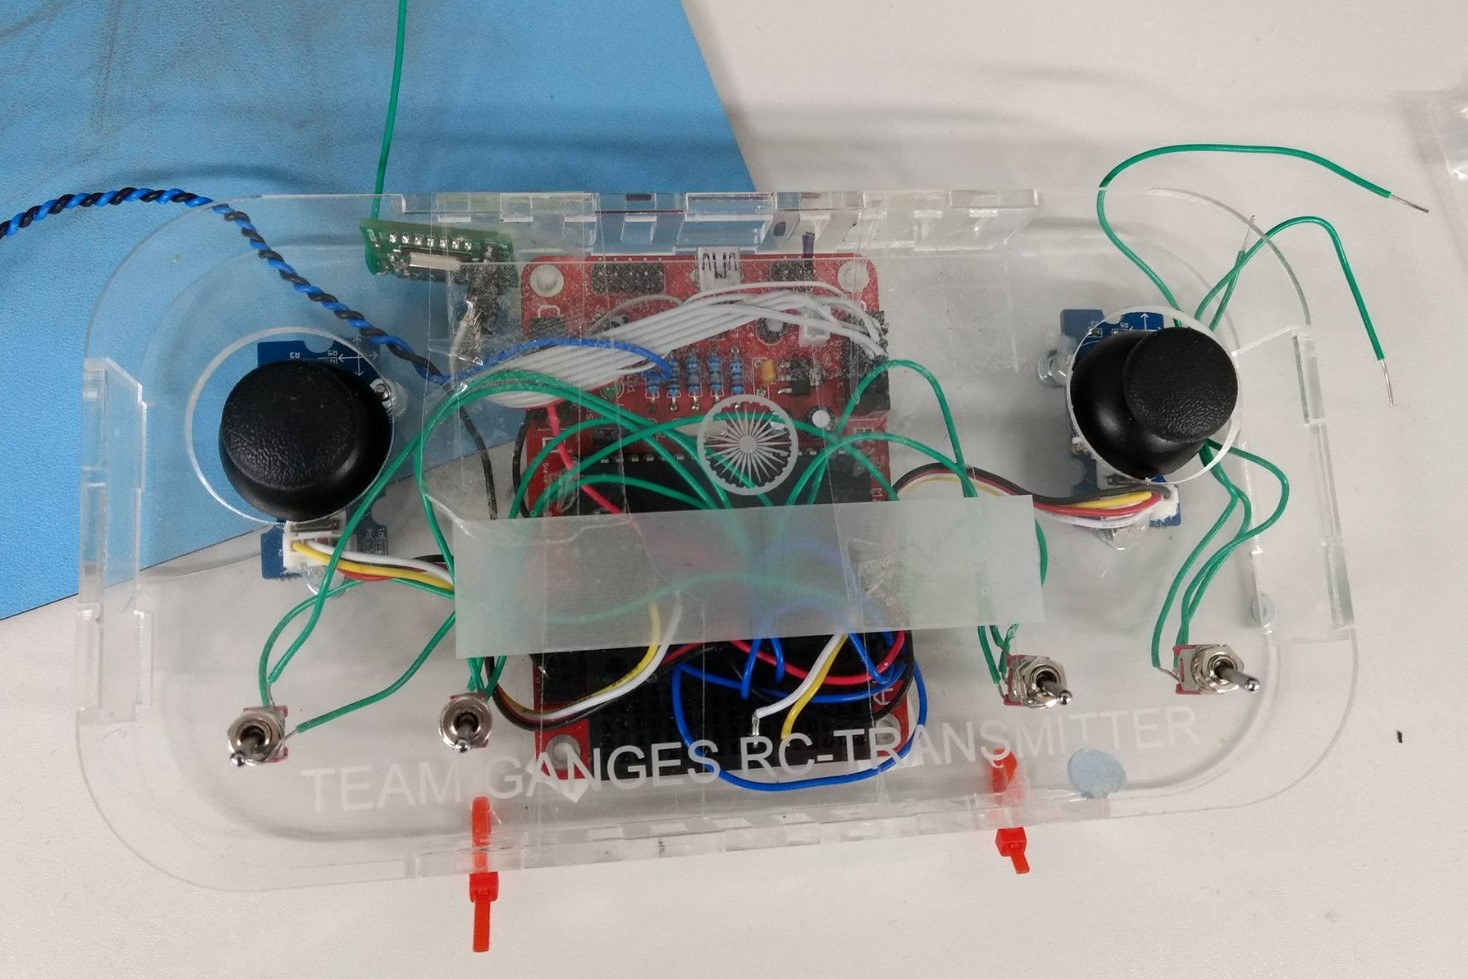
\includegraphics[width=0.9\linewidth, height=5cm]{remote.jpg} 
    \caption{Final build of the Human drone interface controller with implemented electronics inside an acrylic casing.}
    \label{fig:subim1}
    \end{subfigure}
    \begin{subfigure}{0.5\textwidth}
    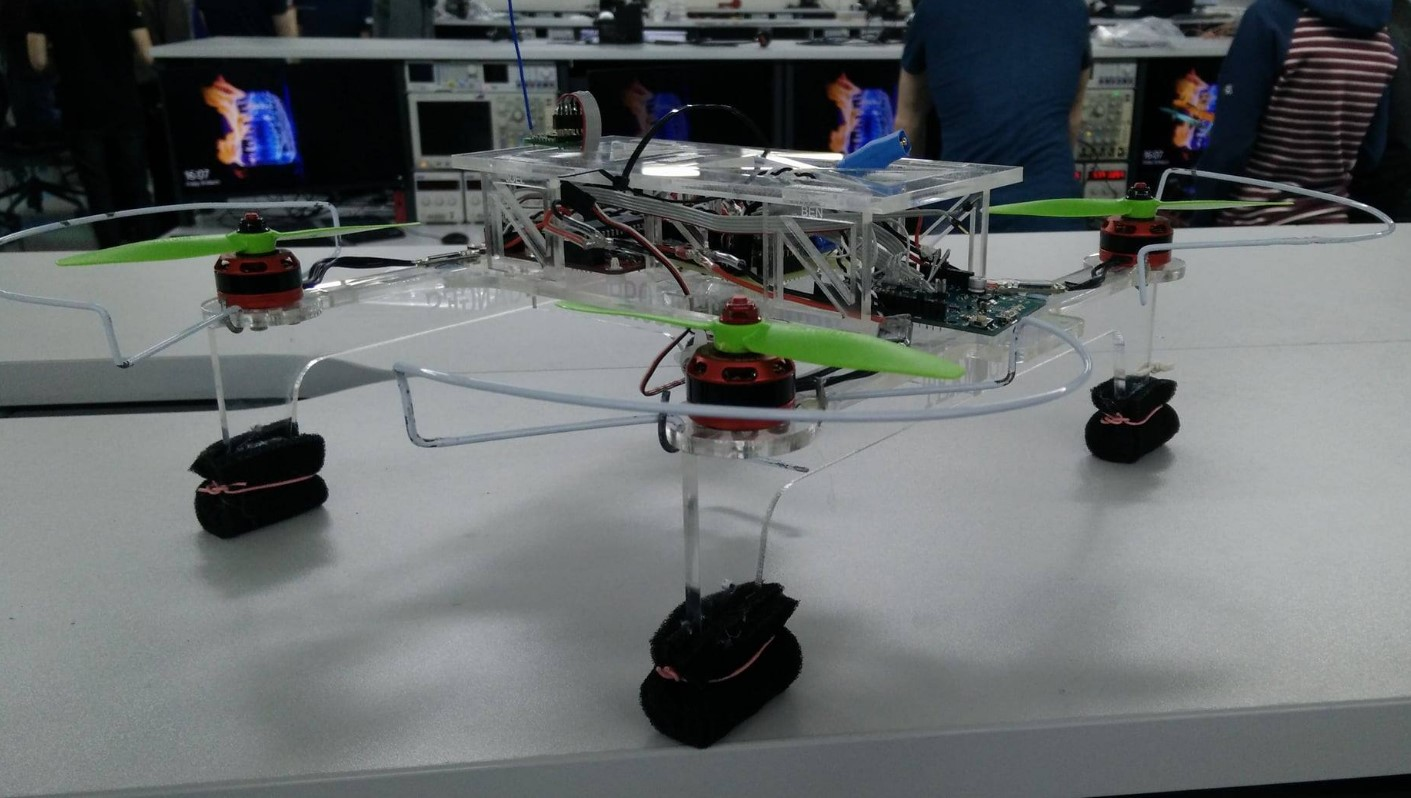
\includegraphics[width=0.9\linewidth, height=5cm]{drone.jpg}
    \caption{Final build of the Quad copter drone consisting of the electronics based on design and specifications, moulded on to the main chassie design.}
    \label{fig:subim2}
    \end{subfigure}
    \caption{Final product images}
    \label{fig:my_label}
\end{figure}
\section{Working of the Final Product}
The remote controller interface consist of joystick potentiometers which are read into the Il Matto using Analogue to Digital converter (ADC) interface. The values are then sent through SPI interface to the RF transceiver modules for wireless up-link of the joystick values to the drone. The RF transceiver on the drone then sends the received values to the Il Matto on the drone through the same SPI interface. The same Il Matto on the drone then sends these values to the Arduino Leonardo through UART interface. Finally the received joystick values in the Leonardo get translated to the corresponding PWM output signals for controlling the speed of the 4 motors. A stabilization controller program is used in the Leonardo which reads the data from the accelerometer/gyroscope sensor as feedback to ensure that the drone maintains stable flight. 
The serial cable in the remote controller is used to view telemetry of the battery voltage on the drone and the IR sensor data through a serial terminal on the PC, when one of the switches is in 'flight mode'. This switch also allows you to enter PID values for yaw, pitch and roll for tuning the stabilization program on the drone when in 'PID mode'.
\section{Extensions}
\begin{itemize}
    \item One of the features that was not achieved was the logging of telemetry data on to the SD card which could have been achieved if we were provided more time for it. We are able to collect live data over the communications interface though. 
    \item Instead of using the PC as a User Interface for telemetry and PID tuning, a TFT screen could have been implemented to make the User interface more localised to the remote.
    \item Being able to overcome the limitation of the User interface for entering different range of PID values and able to tune the stabilization controller on the drone during its flight.
    \item Adding IR sensors to the front and bottom of the drone to allow it to detect obstacles and control its motors accordingly to avoid collision.
    \item Implementing an auto landing feature for the drone to use the bottom IR sensor to land itself safely. The 4th switch on the remote was meant to enable this operation, where when switched on, the drone would reject control commands from the controller and would self land onto ground by accordingly adjusting its motor speed to ensure secure landing.
\end{itemize}
\end{document}